\documentclass[prl,twocolumn]{revtex4-1}
\usepackage{graphicx}
\usepackage{amsmath}
\usepackage{hyperref}
\usepackage{booktabs}
\usepackage{xcolor}

\usepackage{siunitx}

\setlength{\tabcolsep}{10pt}

\newenvironment{sistema}%
  {\left\lbrace\begin{array}{@{}l@{}}}%
  {\end{array}\right.}



\begin{document}
\title{Gelation as a condensation frustrated by hydrodynamics and mechanical tension}
\author{Hideyo Tsurusawa}
\thanks{These authors contributed equally to this work}
\author{Mathieu Leocmach}
\thanks{These authors contributed equally to this work}
\author{Hajime Tanaka}
\email{tanaka@iis.u-tokyo.ac.jp}
\affiliation{ {Institute of Industrial Science, University of Tokyo, 4-6-1 Komaba, Meguro-ku, Tokyo 153-8505, Japan} }

\begin{abstract}
A colloidal gel is an important non-ergodic state of matter with a heterogeneous structure, which can have mechanical elasticity and fluidity at the same time. This coexistence of solid and fluid properties is unique to gels and crucial in many applications. Colloidal gels are known to be formed by phase separation accompanying dynamical arrest of a colloid-rich phase due to glass transition. Even at a low colloid volume fraction, the system forms a space-spanning network structure. Using confocal microscopy, we follow the entire process of gelation from the very beginning with a single-particle resolution for the first time. We switch off long-range Coulomb interactions between charged colloids by injecting salt at $t=0$ through an osmotic membrane and make depletion attractions due to polymers operative. This initiates phase demixing without inducing disturbing flow, which is inevitable for a conventional method, i.e., simple mixing of colloids and polymers at $t=0$. Our method allows us to experimentally access the role of hydrodynamics in the formation process of a percolated network structure. We also succeeded in experimentally revealing an elementary coarsening process of a network, i.e., mechanical-tension-induced breakup of a network and the resulting network coarsening. Thus, we clarify the roles of hydrodynamics and mechanics in gelation, which has not been accessed experimentally. This would contribute to our fundamental understanding of the physical mechanism of gelation and its structural formation.
\end{abstract}

\maketitle

\section*{Introduction} 



\section*{Results}

\subsection*{System design}

\begin{figure*}
	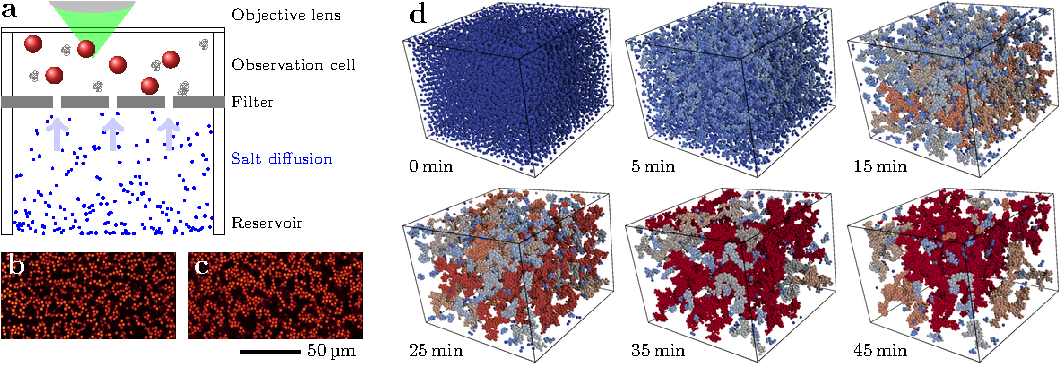
\includegraphics{figs/cell_vs_cap2.pdf}
	\caption{\textbf{Reservoir cell.} \textbf{a} Sketch of our experimental setup. The observation cell contains initially colloids, polymer and no salt. \textbf{b} Confocal slice of a gel formed \textit{in situ} by our method ($\phi=25.5~\%$, $c_p=\SI{1.4}{\gram\per\litre}$), \SI{1}{\hour} after gelation. \textbf{c} Idem for a gel at the same state point formed \textit{ex situ} and immediately pumped into a capillary. \textbf{d} Gelation observed by our method. Experimental coordinates are reconstructed and coloured by the number of particles in clusters in a typical sample close to the cluster-gel line ($\phi=7.5~\%$, $c_p=\SI{1}{\gram\per\litre}$). Origin of time is the last frame before melting of Wigner crystal.
	%Phase diagram obtained in reservoir cell. Spinodal line is obtained from free volume theory. State points analysed in the text are circled. The state point of \textbf{b-c} is highlighted by a square.
	}
	\label{fig:cell_vs_cap}
\end{figure*}

We designed an experimental set-up that allows the observation of the entire process of gelation at a single particle level. For that, we use a colloidal system that is charge stabilised at long range, has a short range depletion attraction, and is also sterically stabilised causing nearly hard sphere repulsion at contact. We disperse colloidal particles and non-adsorbing polymers in a  mixture of organic solvents that matches both the refractive index and the density of the particles. In such weakly polar solvent, here dielectric constant $\epsilon_r = 5\sim6$, Debye screening length is about $\kappa^{-1}=\SI{10}{\micro\metre}$, enough to keep apart even the large colloids suitable for particle-level confocal microscopy~\cite{Royall2003}, here diameter $\sigma=\SI{3}{\micro\metre}$. The short ranged, $\sigma/10$, depletion attraction caused by the polymers is masked by the electrostatic repulsion.

We enclose the suspension in a thin microscopy cell sketched in Figure~\ref{fig:cell_vs_cap}a. The bottom wall of the cell is an osmotic membrane providing contact with a long channel full of the same solvent mixture. We introduce solid salt at the other end of the channel that we seal immediately. Salt dissolution and subsequent migration of the ions along the channel and through the membrane induce screening of the electrostatic repulsion, revealing the depletion potential well. The time needed for the ions to diffuse from the membrane across the cell thickness is of the same order of magnitude as the Brownian time of the particles $\tau_B=\SI{10}{\second}$. This method causes uniform gelation without any solvent flow and allows \textit{in situ} confocal microscopy observation throughout the process.

In Figure~\ref{fig:cell_vs_cap}b and c we show confocal microscopy images of the final structures for two gels prepared at the same state point, one by our protocol, the other by introducing in a capillary an existing gel and thus shear melting it. The later is coarser, highlighting that shaking or shear melting protocols~\cite{lu2008gelation,Teece2011,Bartlett2012} are not equivalent to a quench. However even in our case we expect differences compared to a quench simulated via molecular or Brownian dynamics, because of the presence of a solvent mediating hydrodynamic interactions~\cite{Furukawa2010}. Thus our protocol might be very close to application relevant processes where the sudden addition of a component (e.g. salt, acid, depletion agent) induces aggregation in an otherwise stable suspension (e.g. milk).

In Figure~\ref{fig:cell_vs_cap}d shows a computer reconstruction from experimental coordinates of a typical gelation experiment at a relatively low volume fraction ($\phi=7.5\%$). Immediately before ions enter the cell ($t=0$), the suspension is in a Wigner crystal state where the particles are far apart due to long range repulsion. As soon as the charges are screened, the particles begin to aggregate and form clusters that progressively connect to each other while coarsening to finally percolate through the field of view at $t=\SI{35}{\minute}$.


\subsection*{Observation of the initial stage}

\begin{figure}
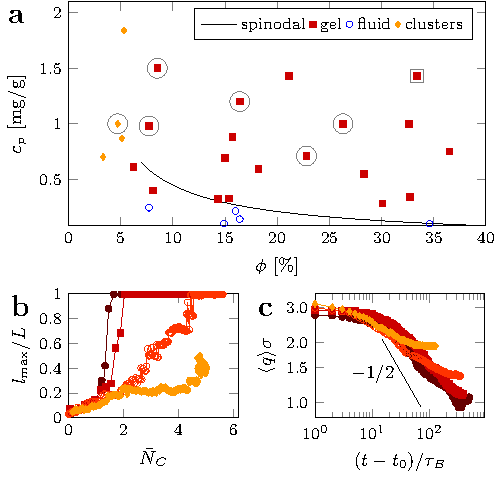
\includegraphics{figs/phasediag.pdf}
\caption{\textbf{Different regimes of gelation.} \textbf{a} Phase diagram. Experimental points are categorised based on the final state obtained in reservoir cell. The spinodal line is obtained from free volume theory. State points analysed in the text are circled. The state point of Figure~\ref{fig:cell_vs_cap}b-c is highlighted by a square. \textbf{b} Comparison of system evolution in terms of largest cluster extent and of mean coordination number. By increasing density: $\phi=4.2,\,8,\,16,\,27~\%$, $c_p=1,\,1.5,\,1.2,\,\SI{1}{\gram\per\litre}$ for \textcolor{red!40!yellow}{$\blacklozenge$}, \textcolor{red!80!yellow}{$\circ$}, \textcolor{red!80!black}{\tiny$\blacksquare$} and \textcolor{red!40!black}{$\bullet$} respectively. \textbf{c} Growth of the characteristic wave number for the same samples.}
\label{fig:phasediag}
\end{figure}


In Figure~\ref{fig:phasediag}a, we divide the phase diagram in three regions based on the final state obtained by our protocol: at low polymer concentration ($c_p<\SI{0.2}{\gram\per\litre}$) sample fully relax to a fluid state; at very low colloid volume fraction ($\phi<0.05$) and high polymer concentration the particles condense into long-lived well separated clusters as observed in~\cite{Lu2006}; in the rest of the explored phase space we observe a long-lived space spanning network. As observed by others~\cite{Shah2003,Bergenholtz2003,lu2008gelation}, the theoretical spinodal line obtained by generalised free volume theory~\cite{Fleer2008} is a poor predictor of the gel boundary, especially at low volume fraction.



With our technique we can observe the path leading to the final state. To characterise this path, we compute the instantaneous mean number of neighbours $\bar{N}_C$, or coordination number that quantifies the compacity of the structure. We also compute the the spatial extent of the largest cluster $l_\text{max}$ that we normalize by the size of the field of view $L$ to obtain a measure of the distance to percolation of the system. Figure~\ref{fig:phasediag}b shows system trajectory in the $(l_\text{max}/L, \bar{N}_C)$ plane for various colloidal volume fractions. At high densities, percolation takes place first, within the first few $\tau_B$ after charge screening and then coarsening proceed. At low densities, percolation never takes place and we observe the compaction of individual clusters. In between, we observe the process detailed in Figure~\ref{fig:cell_vs_cap}d: formation of low-compacity clusters that then slowly connect together to build the percolating network. This process can take hundreds of $\tau_B$ and is competing with cluster compaction, as indicated by the oblique trajectory in Figure~\ref{fig:phasediag}b. The path to gelation is thus not universal and depends on the colloid volume fraction even within the gel region.

The initial similarity between the trajectories of dilute gels and cluster phase is striking, as if their dynamics were ruled by the same phenomenon. To confront this hypothesis, we compute the time dependent static structure factor $S(q,t)$. For all gel and cluster samples we observe the appearance of a low $q$ peak in $S(q)$, see Supplementary Figure XXX, which is characteristic of spinodal decomposition in a system of a conserved order parameter. To track the position of this peak, we compute the characteristic wave number $\langle q \rangle$ and show its temporal evolution in Figure~\ref{fig:phasediag}c. The curves for all samples follow a master curve coherent with spinodal decomposition kinetics: at short times $\langle q \rangle(t)$ shows a plateau indicating that the low $q$ peak builds up at constant wave number corresponding to distances of about $2\sigma$, whereas at intermediate times we observe coarsening with $\langle q \rangle \sim t^{-1/3}$. Finally at longer times each sample deviates from the master curve to form a plateau indicating arrest. The more dilute samples arrest sooner.

Our observations indicate that both cluster and gel phases are due to an arrested spinodal decomposition: network-type spinodal for the gel, and droplet-type spinodal for the clusters where the initial state is too far from equicomposition to allow a bicontinuous structure.

Two questions remain, corresponding respectively to the dilute or dense routes to gelation: (i) How can individual clusters percolate a long time after their formation? (ii) How does a percolated network evolve toward more compact states? We will show that the answers come from mechanical effects: respectively hydrodynamics and internal stresses.

\subsection*{Role of hydrodynamics}

\begin{figure}
	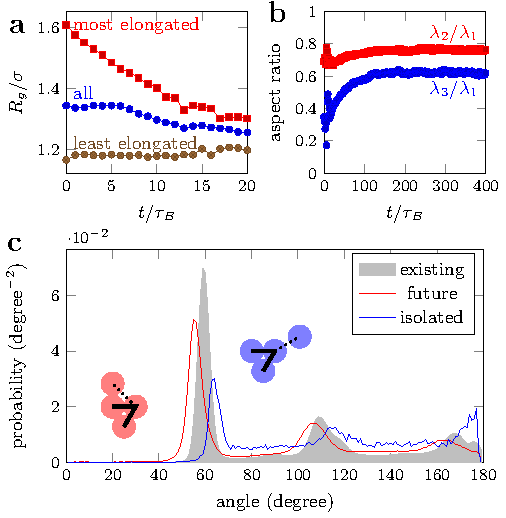
\includegraphics{figs/hydro.pdf}
	\caption{\textbf{Hydrodynamics} \textbf{a} Probability of staying elongated for a triplet in a non percolating sample ($\phi=4~\%$, $c_p=\SI{1}{\gram\per\litre}$). The continuous line is the best exponential fit of characteristic time $27\tau_B$. Inset: probability distribution of radii of gyration of triplets. \textbf{b} Evolution of the aspect ratios of clusters of 4 particles and more in the same sample (dashed lines) and in a percolating sample ($\phi=8~\%$, $c_p=\SI{1.5}{\gram\per\litre}$, continuous lines) \textbf{c} Bond angle distribution relative to existing bonds (gray), to a future bond (red) or to a future bond involving an isolated particle (blue) obtained in the percolating sample. Future bonds are shifted to smaller angles, whereas gas adsorption takes place from larger angles. Insets sketch both cases, with present bonds drawn thick and future bonds drawn dotted.}
	\label{fig:hydro}
\end{figure}


In Figure~\ref{fig:hydro}a, we follow the compaction of clusters made of only three particles in a non percolating sample. The probability distribution of the radius of gyration $R_g$ of these triplets shows two peaks on both sides of $R_g^*=0.8\sigma$. For $R_g<R_g^*$ the cluster is compact, with a structure close to an equilateral triangle. For $R_g>R_g^*$ the three particles are aligned and the cluster is elongated. We found that just after the quench most triplets are elongated and then either connect to other clusters or relax to the more stable compact state. To follow this relaxation, we define the probability to stay elongated as
\begin{equation}
P_\text{el}(\Delta t) = \left\langle P\left(\delta_i(t+\Delta t)|\delta_i(t)\right)\right\rangle_{t,i}
\end{equation}
where $\delta_i(t)$ is the probability for the triplet $i$ to be elongated at time $t$. The decay of $P_\text{el}(\Delta t)$ has a characteristic time of $27\tau_B$, much longer than the Brownian time. 

The shape of clusters of more than 3 particles cannot be followed in the same way. We compute the principal moments of gyrations $\lambda_j$ with $\lambda_1\geq\lambda_2\geq\lambda_3$. Low values of the aspect ratios $\lambda_2/\lambda_1$ and $\lambda_3/\lambda_1$ indicate that the cluster is flat or even linear. In Figure~\ref{fig:hydro}b, we show the evolution of the average value of these aspect ratios either for a non-percolating sample or before percolation for a percolating one. In both cases, we observe that the clusters are originally not compact and become more isotropic over tens of $\tau_B$. As visible in Figure~\ref{fig:cell_vs_cap}d, isotropy is recovered by the fusion of many anisotropic clusters into a branched structure. 




These observations can be rationalised by the invocation of hydrodynamic effects. Indeed in a solvent, particles cannot converge freely to form compact structures~\cite{Furukawa2010}. The compaction is delayed by the incompressibility of the solvent. Furthermore, clusters influenced by hydrodynamic interactions tend to be more elongated, less compact. We can test this hypothesis by measuring at which angle particles meet relative to existing neighbours. If influenced by hydrodynamics, particles should avoid the direction of existing neighbours and come from more open angles.

In Figure~\ref{fig:hydro}c we show the bond angle distribution from three points of view: (i) existing bonds, (ii) bonds that will form within the next $\tau_B$ (iii) bonds that will form within the next $\tau_B$ involving a isolated particle. As expected, existing bonds are preferentially at a \SI{60}{\degree} angle indicating stable packing, with secondary peaks coherent with a mixture of tetrahedral and hexagonal packings. Future bonds have more acute angles and almost never \SI{180}{\degree}, since they are mostly due to particles attached to second neighbours, see sketch on Figure~\ref{fig:hydro}c. Here hydrodynamics plays no role. By contrast, future bonds involving isolated particles form at more obtuse angles, with a clear peak around \SI{180}{\degree}. This confirms that hydrodynamics influences particle aggregation and explains why clusters are initially elongated.

Consequently, long-lived elongated clusters have a higher probability to meet via either rotational or translational diffusion than compact spherical clusters. In Supplementary Figure~\ref{fig:effectiveVF} we show that indeed at all colloidal volume fraction percolation takes place when the effective volume fraction $\phi_\text{eff} = \sum\frac{4\pi}{3}R_g^3$ of the clusters reaches random close packing. Hydrodynamics explains why in a rather dilute regime we can observe immediate formation of elongated clusters and then their slow, diffusion limited aggregation into a percolated structure.

\subsection*{Network ageing}

\begin{figure*}
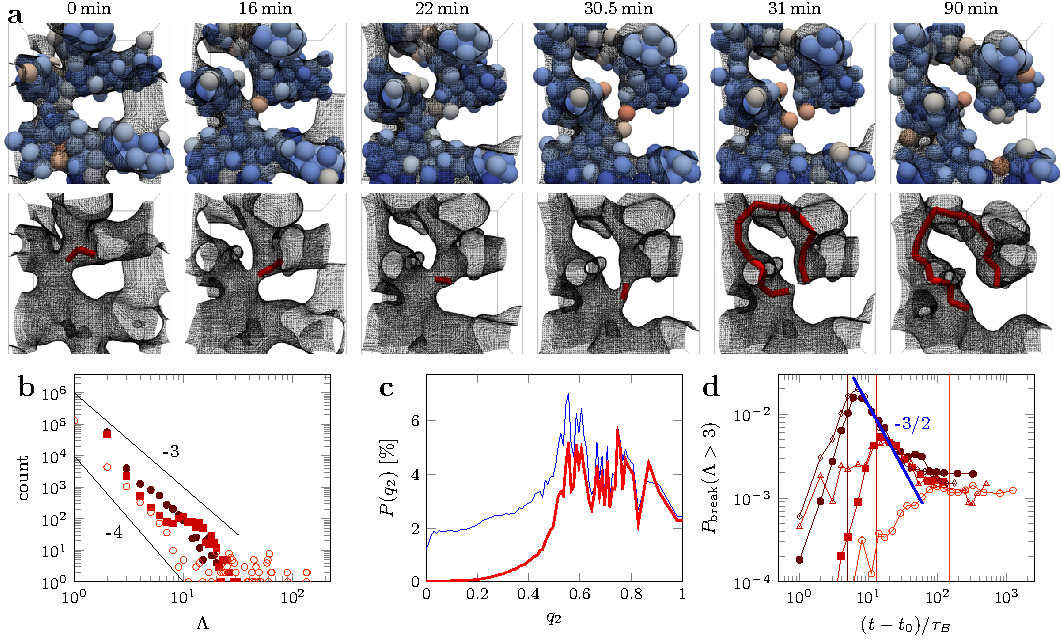
\includegraphics{figs/breaking.pdf}
\caption{\textbf{Mechanical tension drives coarsening} 
\textbf{a} Reconstruction from experimental coordinates ($\phi=29~\%$, $c_p=\SI{0.7}{\gram\per\litre}$) of coarsening process geometry (top) and topology (bottom). Particles are drawn to scale and coloured by $q_2$ from blue (low) to red (high). The meshed surface is a Gaussian coarse-graining of the network pattern. The red line indicates the shortest on-graph path between the two particles of interest. 
\textbf{b} Number of bond breaking function of the future on-graph distance $L$ (after percolation) for the three percolating state points of figure 2 (same colours and markers).
%three state points of increasing density: $\phi=8,\,16,\,27~\%$, $c_p=1.5,\,1.2,\,\SI{1}{\gram\per\litre}$ for \textcolor{red!80!yellow}{$\circ$}, \textcolor{red!80!black}{\tiny$\blacksquare$} and \textcolor{red!40!black}{$\bullet$} respectively.
\textbf{c} Probability for a bond to break during $3\tau_B$ function of bond-centred $q_2$ for all events (blue) and for events with $L>1$ (thick red) in the same sample as \textbf{a}.
\textbf{d} Evolution of the topologically relevant bond breaking probability ($L>3$) for the same state points  as in b. Vertical lines indicate the respective percolation times.
}
\label{fig:breaking}
\end{figure*}

We now change our focus to percolated samples. As we saw in Figure~\ref{fig:phasediag}c, the coarsening in these samples is much slower than what is expected from spinodal decomposition dynamics. The phase separation is arrested, but the system is still ageing, a process sometimes leading to delayed sudden collapse of gels~\cite{Teece2011,Bartlett2012}, a catastrophic phenomenon from the industrial point of view. Previous studies~\cite{Tanaka2007,Bartlett2012} have shown that the main coarsening mechanism is the rupture of strands in the network, a process that to our knowledge has not been followed experimentally at the particle level.

Figure~\ref{fig:breaking}a shows a strand rupture reconstructed from confocal 3D images, the colours mapping the intensity of internal stresses acting on each particle. In practice, the attraction potential well is too narrow relative to the particle localisation errors for us to extract directly the force acting on a particle. Therefore, we use the elongation of the particle neighbourhood as a proxy. The more the bonds around a particle are oriented along a single axis, the more tension is exerted on the particle. This local elongation is quantified using~\cite{steinhardt1983boo} bond orientational order for the 2-fold symmetry $q_2$, see Methods for a precise definition. On Figure~\ref{fig:breaking}a we observe the slow build up of tension over the first \SI{30}{\minute}, until the tension is concentrated on a one particle thin strand. This strand breaks and the particles involved merge in their respective part of the network that then stay apart from each other.

To detect strand rupture, we use the topology of the bond network. We can consider the gel as a graph with the particles as nodes and the bonds as edges. This graph evolves from frame to frame separated by $3\tau_B$. In the lower part of Figure~\ref{fig:breaking}a we draw in red the shortest on-graph path between two particles of interest. Before the strand rupture, this path is a single bond long. After the rupture, the shortest path is much longer. In general, when two particles were bonded on the previous frame and are no more bonded on the present frame, we define the post-breaking topological distance $L$ as the new shortest distance on the graph between them, minus 1. If the particles still have a common neighbour then $L=1$, because two bonds are needed to go from one to the other. $L=2$ when three bonds are needed, etc.

$L$ is a good measure of the significance of a bond breaking event. Small values indicate a local rearrangement whereas large values are the signature of important changes in the topology of the network, namely strand rupture. Figure~\ref{fig:breaking}b shows the distribution of $L$ for three colloidal volume fractions. Excluding the largest values that are dominated by the limited size of the field of view, $L$ seems to follow a power-law distribution of exponent between $-3$ and $-4$. However the values at $L=1$ seems in excess. Figure~\ref{fig:breaking}c compares the probability distribution of $q_2$ for all bond breaking events versus for evens with $L>1$. In both cases bonds about to break have a higher probability of being under tension, but this trend is much clearer when excluding local events. Both observations point to spurious detection of bond breaking events due to localisation errors comparable to the short attraction range and rattling of particles. For this reason, but also to focus on topologically relevant strand rupture, we discard all events with $L<4$ in the following analysis.

In Figure~\ref{fig:breaking}d we show the time evolution of the probability for a topologically relevant strand rupture $P_\text{break}(L>3)$, i.e. the ratio of the number of bond breaking events with $L>3$ by the number of particles. $P_\text{break}$ is maximum at percolation and then decreases and finally saturates. Strikingly all curves collapse after percolation, indicating common physical ingredients for the ageing of gels at all concentrations.

Initially, clusters are in elongated, unstable configurations. When isolated, a cluster is able to relax to a more compact and stable shape. However in dense samples, elongated clusters meet before any compaction into large branched clusters able to transmit stresses. The compaction trend exerts internal stresses on the strands inside those clusters large enough to make them rupture. This effect is maximum when the sample is fully percolated and thus the internal stresses are maximum.

The characteristic size of a spinodal network is $\xi(t)\sim t^{1/3}$. Strands being linear objects, their volume is linear in $\xi$ and thus the number of strands in the field of view $N_s$ evolves as $t^{-1/3}$. If we suppose that after the percolation no new strands are created, the variation in the number of strands is only given by the strand rupture rate:
\begin{equation}
P_\text{break} = -\frac{d N_s}{dt} \sim t^{-4/3}.
\end{equation}
Indeed in Figure~\ref{fig:breaking}d we observe that the initial regime of the master curve is well described by a power law of exponent $-4/3$. 

At longer times, most of the internal stresses have been released and the system reaches arrested phase separation, where the strand rupture rate becomes comparable to the strand creation rate.

For dilute samples, percolation happens later, after the end of the power law regime. The clusters have already compacted to stable configurations and internal stresses are low.




\section{Conclusion}




\section*{Methods}

\subsection*{Experimental}

We used \textsc{pmma} (poly(methyl methacrylate)) colloids sterically stabilized with methacryloxypropyl terminated \textsc{pdms}(poly(dimethyl siloxane)) and fluorescently labelled with rhodamine isothiocyanate chemically bonded to the \textsc{pmma}. Colloids are dispersed in a mixture of cis-decalin (Tokyo Kasei) and bromocyclohexane (Sigma-Aldrich) that matches both optical index and density of the colloids.

To induce short-ranged depletion attraction, we use polystyrene (TOSOH) of molecular weight \SI{8.4}{\mega\dalton} as non-adsorbing polymer. The radius of gyration in theta solvent is estimated to \SI{110}{\nano\metre}. Here the solvent may be regarded as ``good'' and a Flory scaling of the measurements of~\cite{lu2008gelation} yields $R_g=\SI{148}{\nano\metre}$. In the absence of salt, the Debye length is expected to reach several \si{\micro\metre} and the (weakly) charged colloids experience a long range electrostatic repulsion~\cite{Royall2003}. We confirm that colloids never come close enough to feel the short-ranged attraction and form a Wigner crystal.

The colloids and polymers are contained in an observation cell ($\SI{1}{\milli\metre^2} \times \SI{200}{\micro\metre}$) made of glass in contact with an half-open glass channel approximately 400 larger in volume, via a millipore filter with pore size of \SI{100}{\nano\metre} that allows the salt through but neither polymer nor colloid (see Fig.~\ref{fig:cell_vs_cap}a). The channel is filled with the same solvents at density matching composition. At the beginning of the experiment, solid tetrabutylammonium bromide (Fluka) is introduced to the channel which is immediately sealed to prevent evaporation. Data acquisition starts within \SI{30}{\second} after salt introduction. Our procedure induces practically no solvent flow in the observation cell. We confirmed the presence of undissolved salt several days after mixing, indicating that the observation cell was brought to saturation concentration.

Given the diffusion constants of Bromide and alkyl cation ($6$ and \SI{2e-10}{\metre^2\second^{-1}}~\cite{Campbell2005}), we estimate the characteristic diffusion time of salt from top to bottom of the order of \SI{10}{\second}. Therefore, we reach uniform final salt concentration into the observation cell within only a few Brownian times of the colloids. Indeed we measured a delay of about \SI{1}{\minute} between the aggregation at the bottom and at the top of the cell. We define the initial time of the aggregation process when the maximum of the $g(r)$ jumps from the lattice constant of the Wigner crystal to the hard-core diameter $\sigma$.


We collect the data on a Leica SP5 confocal microscope, using \SI{532}{\nano\metre} laser excitation. The temperature was controlled on both stage and objective lens, allowing a more precise density matching. The scanned volume is at least $82 \times 82 \times \SI{85}{\micro\metre}$. The particle coordinates are tracked in three dimensions (3D) with an accuracy of around $0.03\sigma$~\cite{LeocmachColloids}.


\subsection*{Analysis}

From direct confocal measurement~\cite{Royall2007, Poon2012}, we estimate the hard-core diameter of our colloids ($\sigma=\SI{2.75}{\micro\metre}$) and the range of the interaction potential (that confirmed our scaling of $R_g$ within $1\%$), leading to a polymer-colloid size ratio $q = 2R_g/\sigma = 0.10(6)$. Spinodal line on Fig.~\ref{fig:phasediag}b are calculated from this size ratio using the generalized free volume theory~\cite{Fleer2008}.

In principle the attraction well of the depletion extends to $\sigma+2R_g$, however resolution-dependent tracking imprecisions and systematic errors do not give a precise enough estimate of such short distance. Therefore we consider two particles bonded when their distance is shorter the first minimum of $g(r)$, i.e. \SI{3.55}{\micro\metre}. This defines the bond graph that we analyse using connected components and shortest path analysis algorithms~\cite{Hagberg2008}.


To detect local 2-fold symmetry and thus elongation, we use \citet{steinhardt1983boo} bond orientational order for the particle $i$,
\begin{align}
	q_2(i) =& \sqrt{\frac{4\pi}{5} \sum_{m=-2}^{2} |q_{2,m}(i)|^2 }, \label{eq:ql}\\
	q_{2,m}(i) =& \frac{1}{N_i}\sum_{j=1}^{N_i} Y_{2,m}(\theta(\mathbf{r}_{ij}),\phi(\mathbf{r}_{ij})),
	\label{eq:qlm}
\end{align}
where the $Y_{\ell, m}$ are spherical harmonics and $\mathbf{r}_{ij}$ is one of the $N_i$ bonds involving particle $i$.

\bibliographystyle{naturemag3}
\bibliography{ico_dyn}
\end{document}